\documentclass[12pt]{scrarticle}

\usepackage[utf8]{inputenc}
\usepackage{graphicx}
\graphicspath{{./}}
\usepackage{listings}
\usepackage[colorlinks=true]{hyperref}
\usepackage{amsmath}
\usepackage{lipsum}
\usepackage{caption}
\usepackage{subcaption}
\usepackage{float}

\title{A running Example of Latex}
\author{Daniel Anthes \and Moritz Nipshagen}
\date{} % defaults to today

\begin{document}

\maketitle

\begin{abstract}
    \lipsum[3]
\end{abstract}

\section{I am a section}

\lipsum[1]

\subsection{I am a subsection}

\lipsum[2]

\section{Math}

Here is an inline formula: $e = mc^2$.

One more, but now on a separate line:

$$
\mathcal{N}(x|\mu, \sigma) = \frac{1}{\sigma \sqrt{2\pi}}\exp \left({\frac{(x - \mu)^2}{2\sigma^2}}\right)
$$

Now with multiple aligned formulas:

\begin{eqnarray}
\dot{x_1} &=& -x_2 + x_{2}^3\\
\dot{x_2} &=& -x_1 + x_{1}^3
\end{eqnarray}

Notice that \textit{eqnarray} numbers the formulas. Add a star to disable numbering:


\begin{eqnarray*}
\dot{x_1} &=& -x_2 + x_{2}^3\\
\dot{x_2} &=& -x_1 + x_{1}^3
\end{eqnarray*}

\section{Images}

\begin{figure}[h!]
    \centering
    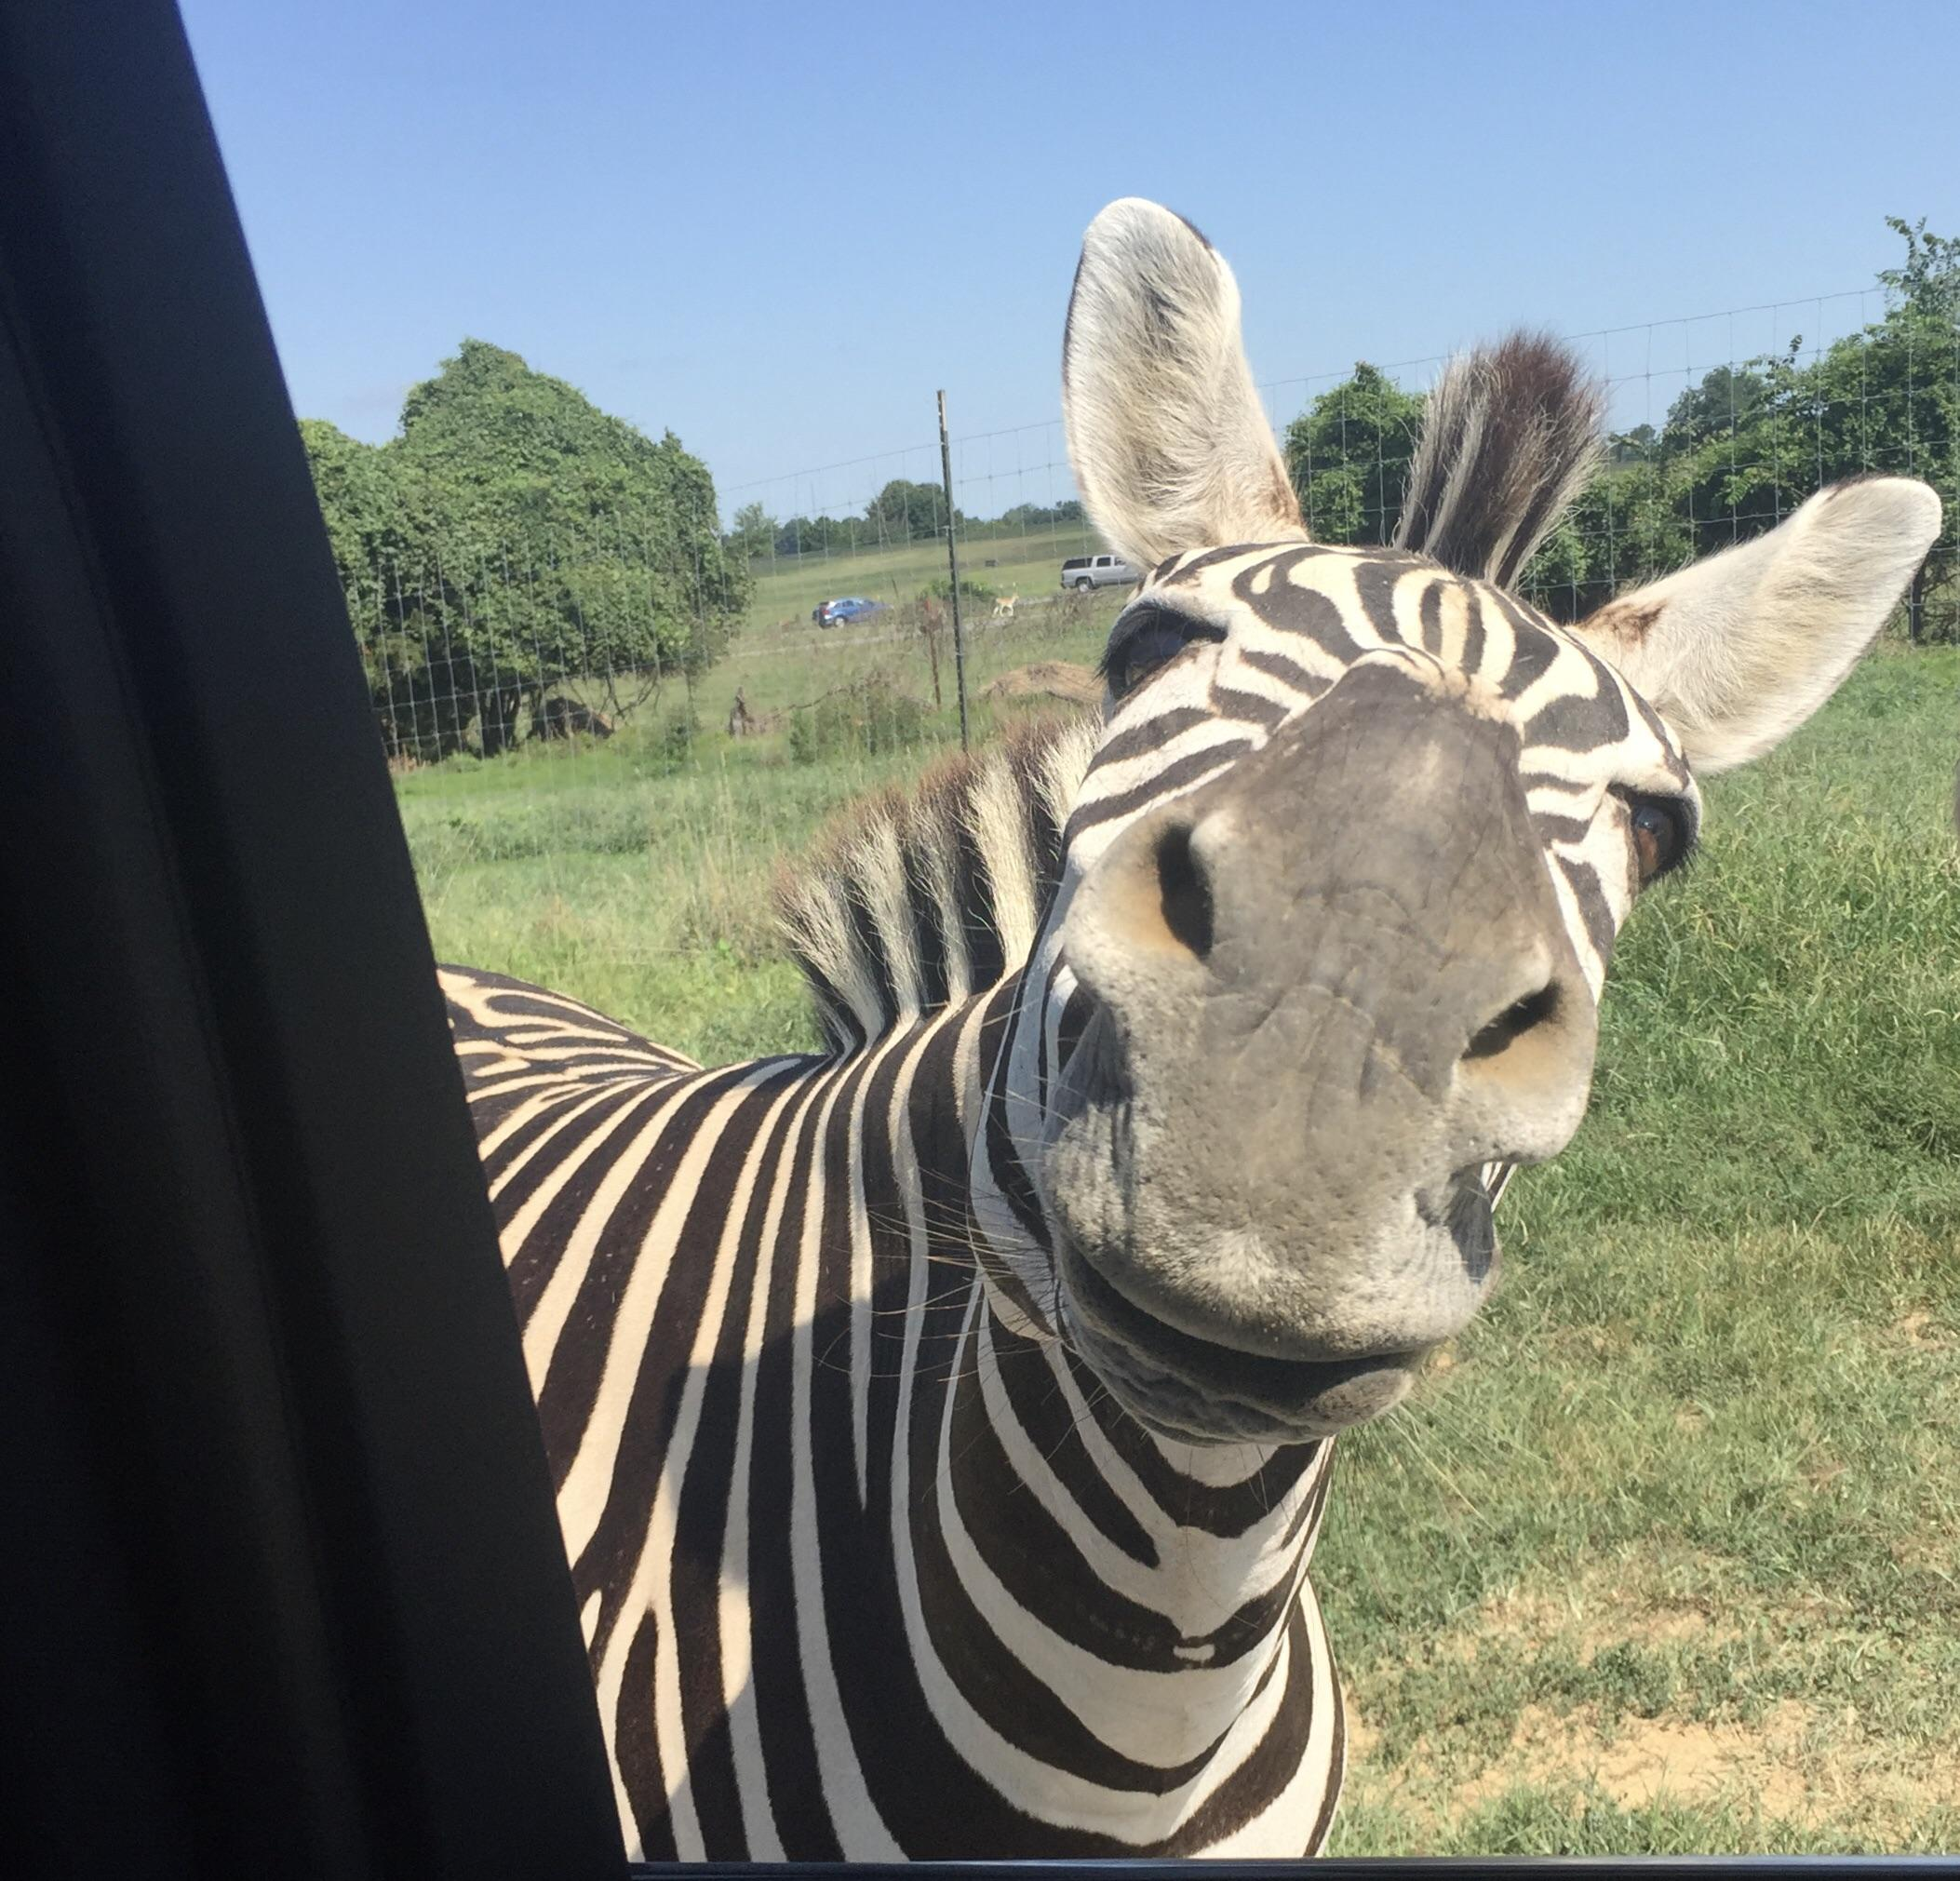
\includegraphics[width=.3\linewidth]{zebra.jpeg}
    \caption{Zebra.}
    \label{fig:examplefig}
\end{figure}

We can also have multiple images in a figure:

\begin{figure}[H]
    \centering
    \begin{subfigure}{0.49\textwidth}
        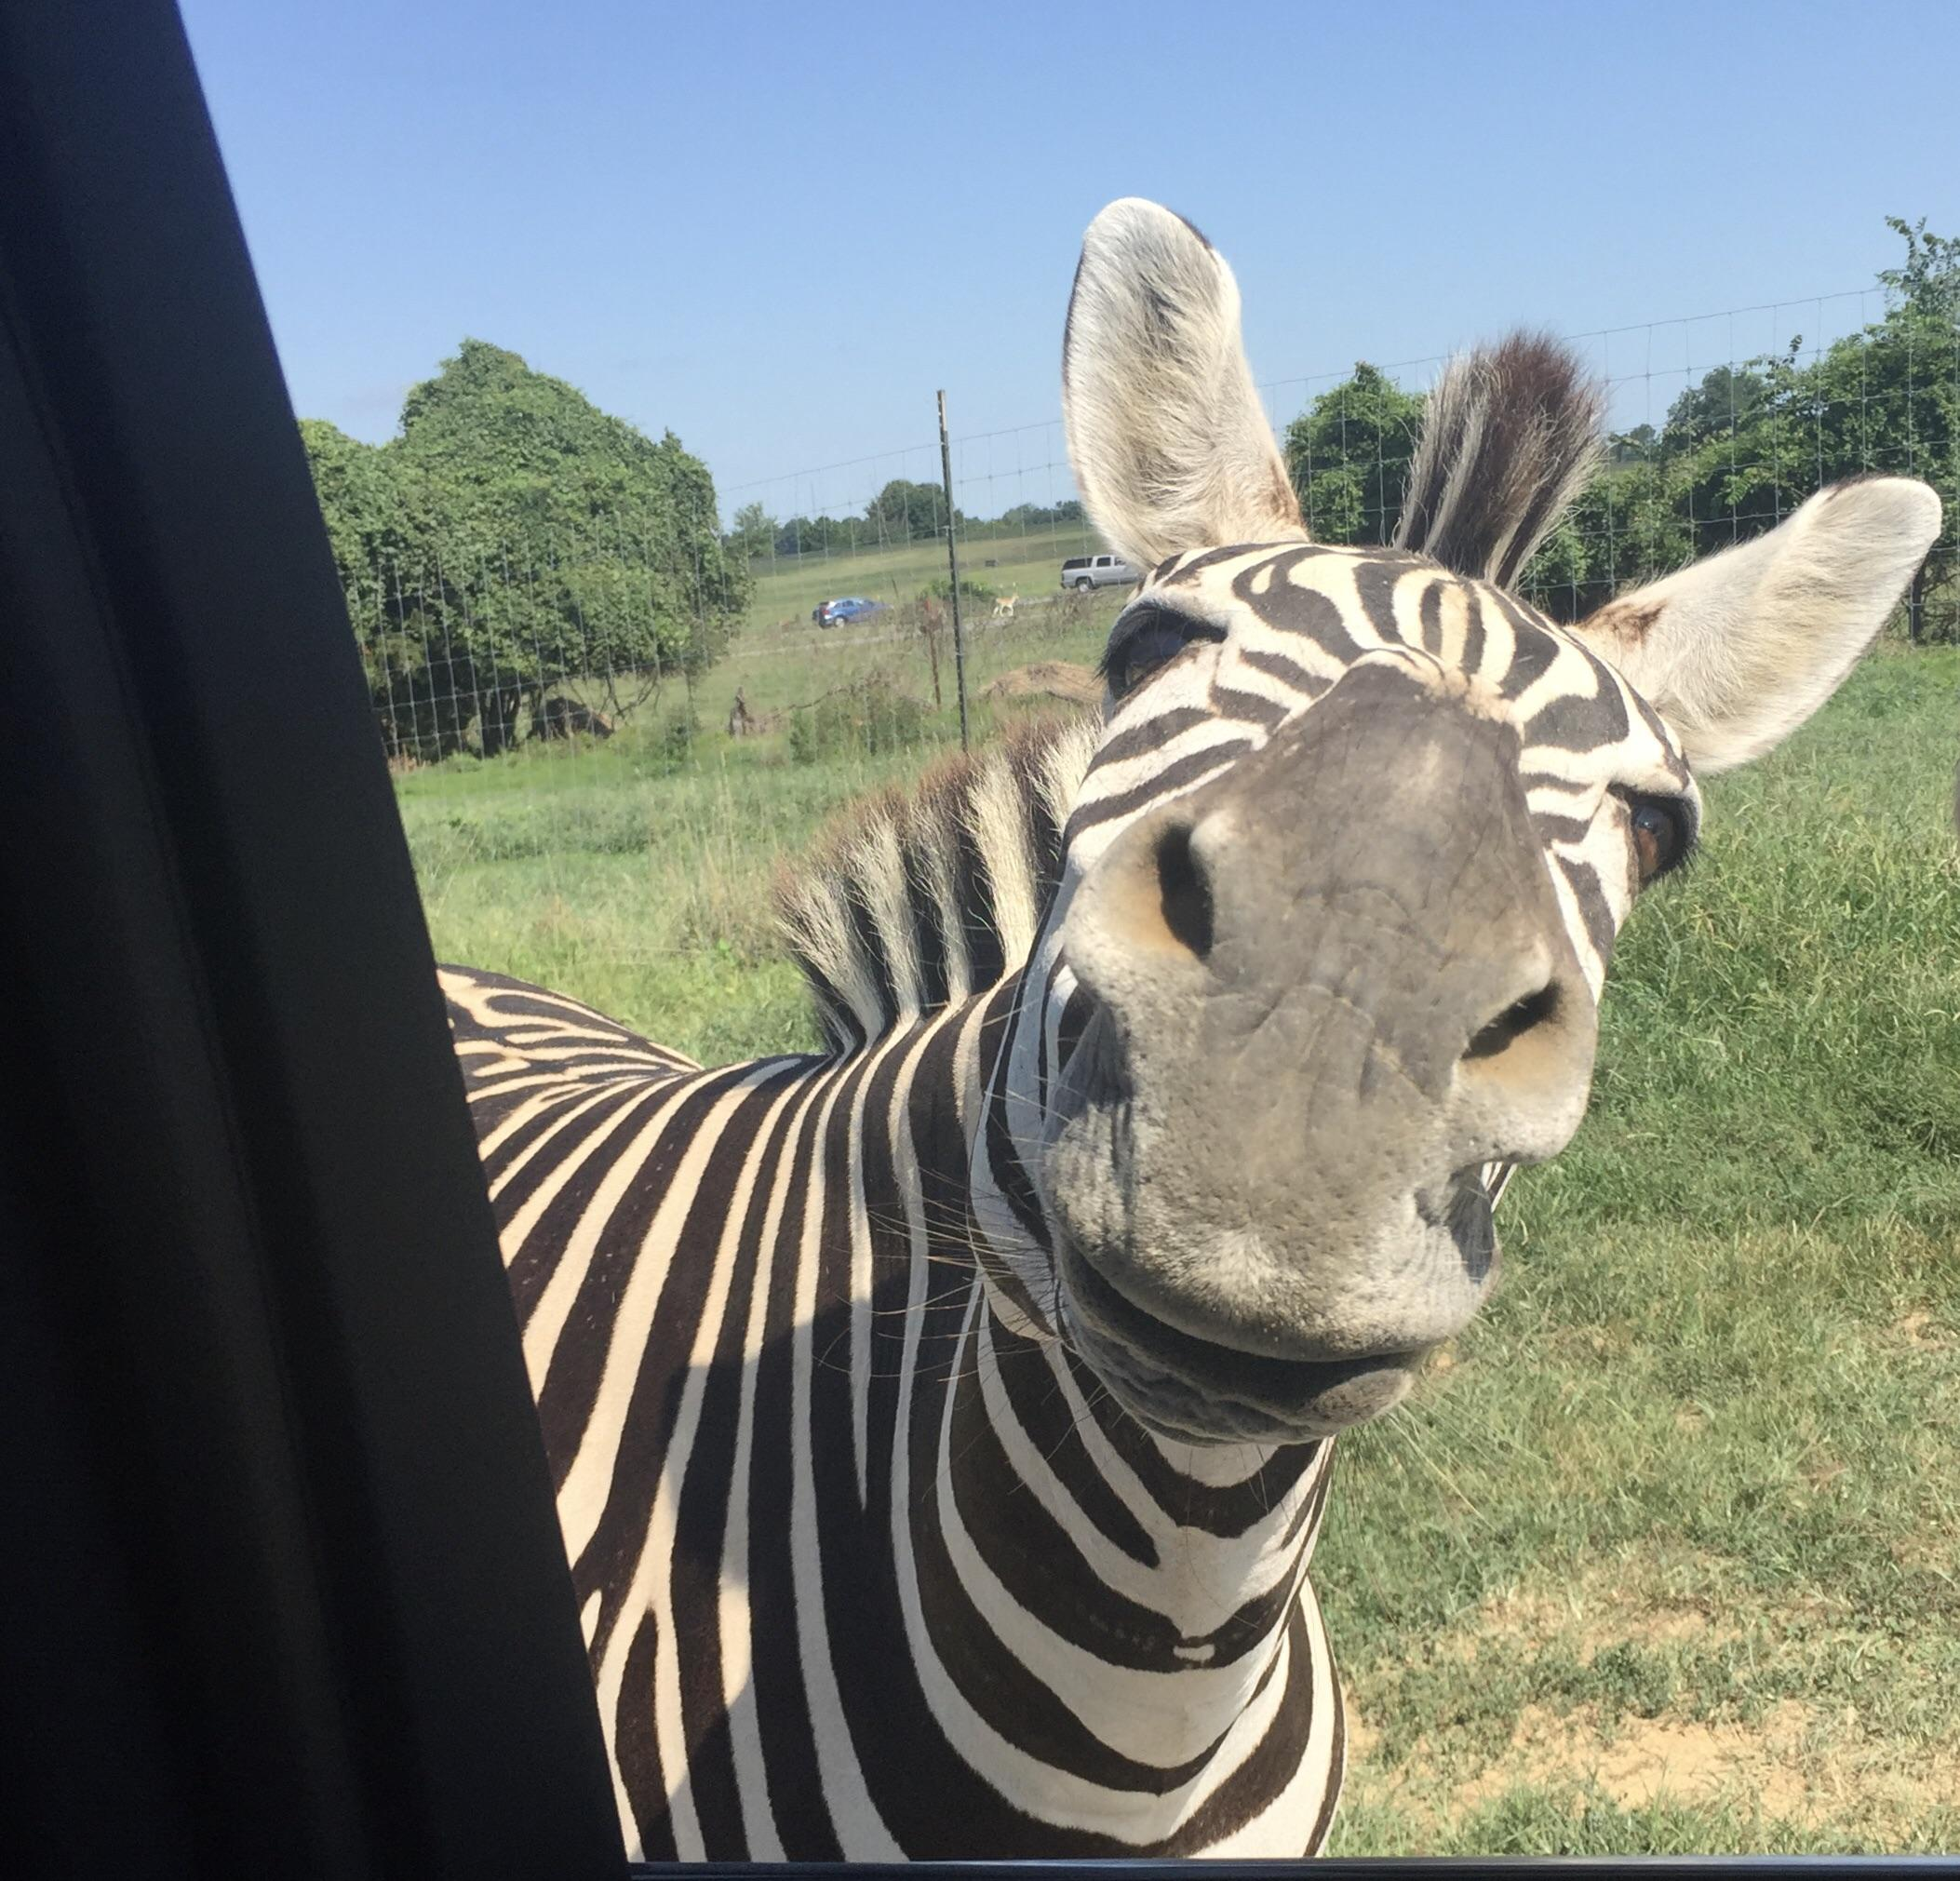
\includegraphics[width=0.9\linewidth]{zebra.jpeg}
        \caption{Zebra.}
    \end{subfigure}
    \begin{subfigure}{0.49\textwidth}
        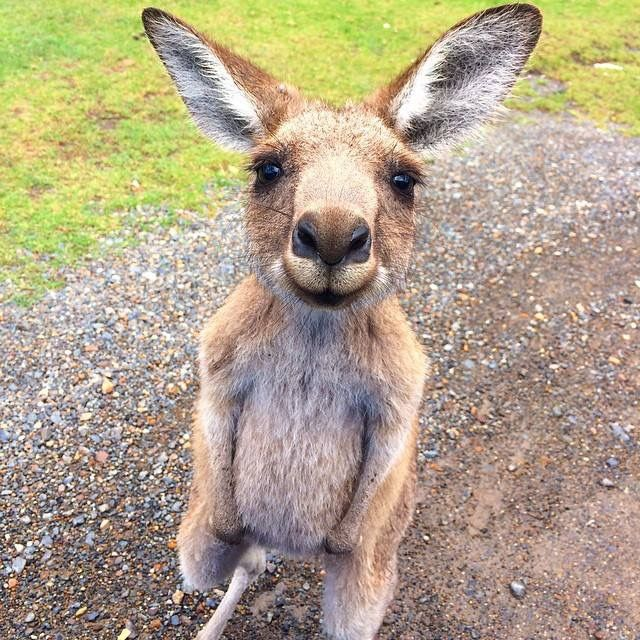
\includegraphics[width=0.9\linewidth]{kangaroo.jpeg}
        \caption{Kangaroo.}
    \end{subfigure}
    \caption{Animals.}
    \label{fig:animals}
\end{figure}

This document contains a lot of figures and not a lot of text. When this happens latex can sometimes have trouble placing the figures and tables in a nice way. We use the \textit{float} package to tell Latex to put figures exactly where we want them. (with the optional argument \textit{H})

\section{Tables}

\begin{table}[H]
    \centering
    \begin{tabular}{|l||c|c|c|}
    \hline 
    Animal & Is Zebra & Is Pet & Legs\\
    \hline\hline
    Dog         & No    & Yes   & 4\\
    Cat         & No    & Yes   & 4\\
    Zebra       & Yes   & No    & 4\\
    Kangaroo    & No    & No    & 2\\
    \hline
    \end{tabular}
    \caption{Animal Facts}
    \label{tab:my_label}
\end{table}

\section{Links, References and Footnotes}

Here is a link: \url{https://dondrite.ruhosting.nl}

And one that has an alternative text: \href{https://www.youtube.com/watch?v=dQw4w9WgXcQ}{A clickable link!}

You can also refer to elements with a label in your document: (\ref{fig:examplefig})

Footnotes are also possible, and clickable\footnote{If you are using the \textit{hyperref} package}

\section{Styling}

You can have \textit{italic} and \textbf{bold} text, \texttt{monospaced} and \textsc{small caps}. Text can also be {\large{large}}, {\Large{larger}}, {\huge huge} and {\Huge really Huge} or {\small{small}} and even {\tiny tiny}.

\begin{center}
    you can center your text as well
\end{center}

And {\color{blue}colors} {\color{red} are} {\color{cyan} also} possible.

Notice that commands such as \textit{color} or \textit{small} affect the rest of the current environment. You can set a "scope" by surrounding the text to be affected by the command with curly braces.

\end{document}